\chapter{Hardware}
\label{hardware}
Hardware selection was approached from a ``minimum sensor" perspective. One of the main goals of this thesis was to reduce the number of sensors as much as possible to increase the variety of aircraft the hardware can fly on. To accomplish this, sensors were chosen based on which state they could estimate, with a main goal being to reduce overall size. The sensors were then combined into a single printed-circuit-board (PCB) that eliminated loose wiring and the potential for error that comes with it. 

\section{Flight Computer}
The flight computer chosen was an Arduino Due. This board has a 32-bit ARM processor, 54 digital I/O pins, 12 analog input pins, and 2 analog output pins. The main driver in the decision to use an Arduino-based platform was the vast support community, which allowed quicker code development. The Arduino also offers a package that integrates well into most of the available airframes, and the stacker head pins allowed for easy integration with other boards. The Due in particular was chosen as it is (at the time of writing) the most advanced Arduino available. The main advantages it has over the comparable Arduino Mega is its increased clock speed (84 MHz for the Due\cite{Atmel2012} vs 16 MHz for the Arduino Mega\cite{Atmel2012atmega}) and its 32-bit architecture (vs. 8-bit for the Arduino Mega). The Arduino Due is also capable of some single cycle floating point arithmetic\cite{Atmel2012}, which is another advantage over the Mega.

\begin{figure}[H]
  \caption{Arduino Due Flight Computer} \label{arduinoPicture}
  \centering
    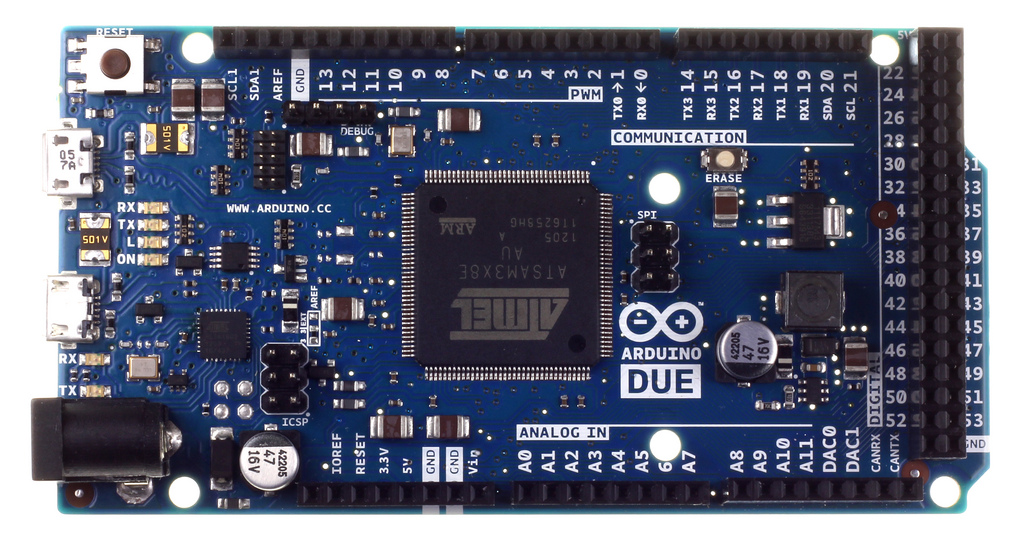
\includegraphics[width=0.5\textwidth]{figures/arduinoDue.jpg}
\end{figure}

The Arduino Due uses a 3.3V architecture instead of the usual Arduino architecture, which uses a 5V operating voltage. This was mainly beneficial, since most of the selected sensors used 3.3V as both supply and logic voltage. An oscilloscope was used to check logic levels of the 5V sensors, and the logical levels were within the Due's voltage limits, so no logic level converters were required. In Due also supplies regulated 5V and passes through the supply power, which must be between 6V and 15V. The board will be powered through the 3.5mm barrel jack, using a 3-cell LiPo battery, with a nominal voltage of 11.1V.

\section{Accelerations}
The accelerometer chosen for this thesis was the ADXL-362 from Analog Devices. It has a noise error of $175\mu\text{g}/\sqrt{\text{Hz}}$ and uses a 3.3V digital SPI interface\cite{adxl362DataSheet}. The accelerometer is in a QFN package and was surface mounted to the main PCB, with a decoupling capacitor between power and ground. The circuit was modeled after Sparkfun's ADXL-362 Breakout Board\cite{Sparkfunadxl362BOB}.
\begin{figure}[h!]
  \caption{ADXL-362 Schematic} \label{adxl362Schematic}
  \centering
    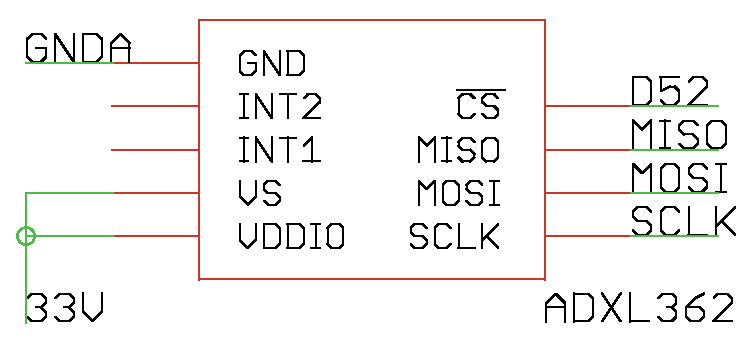
\includegraphics[width=0.5\textwidth]{figures/adxl362.eps}
\end{figure}

Each axis of the accelerometer was calibrated using a two step method. The first step was to orient the axis being calibrated in a direction not influenced by gravity. Data was acquired for 10 seconds and a simple average was taken. This value was then subtracted from every reading to correct for zero offset. The second step was to take two different readings: first, with the positive axis in the gravity direction; and second, with the negative axis in the gravity direction. Both readings were taken after removing the zero offset using step one. A linear line was fit between a nominal $\pm-32.2 \frac{ft}{s^2}$ gravity value.
%todo:include accelerometer calibration curves.
\section{Vehicle Mass}
All test vehicles will be weighed using a U-Line H-1650 counting scale. The scale has an accuracy of 0.001 lbs and a maximum capacity of 30 lbs. The minimum capacity of the scale is 10 grams \cite{U-Line}.
\section{Euler Angles}
The Euler angles of the aircraft can be estimated using either an 3-d electronic compass or a 3-d magnetometer. A magnetometer reads the direction and magnitude of a magnetic field, while a compass combines a magnetometer with accelerometer readings to produce a more accurate estimate of the true angles. However, if the vehicle is maneuvering, the craft's acceleration will distort the angle estimation, making compasses unsuitable for this application. Two separate magnetometers were used for separate purposes. A Honeywell HMR-2300 3-d magnetometer is the main magnetometer and is used for the most accurate sensing possible. 

\begin{figure}[H]
  \caption{Honeywell HMR-2300 3-d Magnetometer } \label{hmr23000Picture}
  \centering
    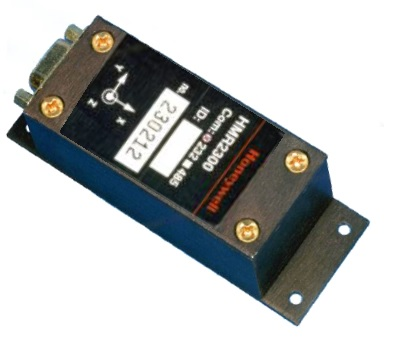
\includegraphics[width=0.5\textwidth]{figures/hmr2300.jpg}
\end{figure}

%todo:take gauss to angles
This magnetometer provides a RMS error of 0.1 milliGauss for all axes, using the 1 Gauss full-scale setting\cite{hmr2300DataSheet}. 

The HMR-2300 can be supplied with power between 6V and 15V, so the 3-cell 11.1V nominal LiPo battery that powers the Arduino also passes through to power the magnetometer. Additionally, the HMR-2300 operates using an RS-232 serial interface. To properly interface with the Arduino Due, which uses 3.3V TTL logic levels, a Max-3232 integrated circuit (IC) was used. This IC, when combined with charge pump capacitors, translates TTL levels between 3V and 5.5V to RS-232 logic levels of $\pm6$V.
 \begin{figure}[H]
   \caption{HMR-2300 Adapter Board Schematic} \label{magBoardSchematic}
   \centering
     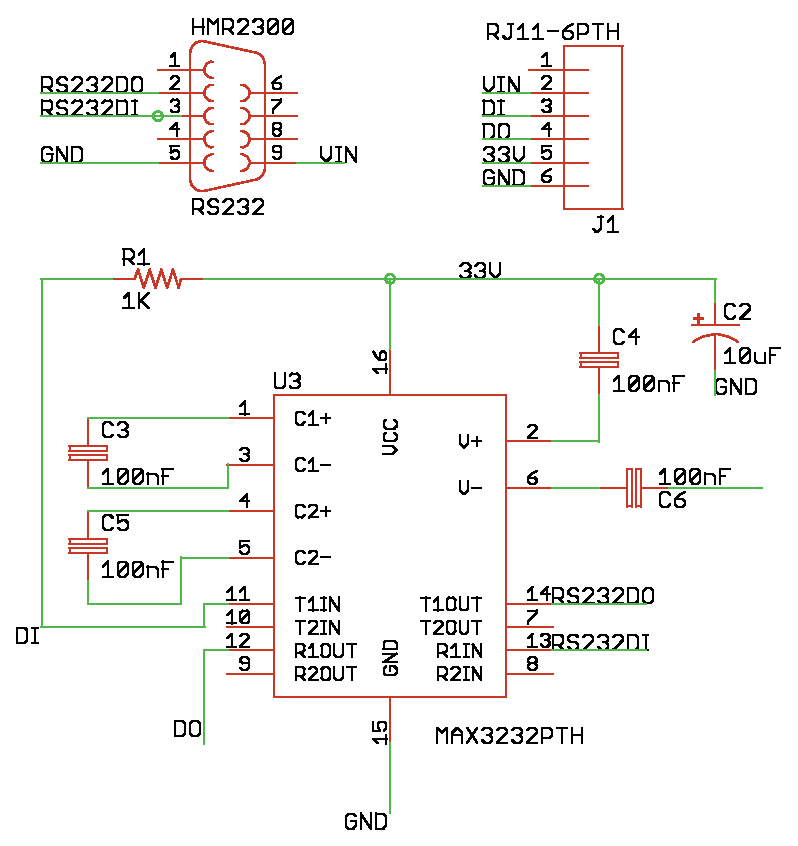
\includegraphics[width=0.5\textwidth]{figures/magBoard.eps}
 \end{figure}
 This board was connected to the magnetometer using a DB-9 connector, and was connected to the flight computer using an RJ-11 cable.\\
 
 The second magnetometer is a Honeywell HMC-5883L, which comes in a QFN package that was surface mounted to the main sensor board. It was added to the system for two main reason: it is much smaller for applications where size is critical, and it is much less expensive for testing with unproven vehicles. It communicates with the Arduino using an I$^2$C interface and uses a 3.3V operating voltage\cite{hmc5883LDatasheet}. The circuit used was similar to that used by Sparkfun on their HMC-5583L breakout board\cite{hmc5883LSchematic}.
 
 \begin{figure}[h!]
   \caption{HMC-5883L Schematic} \label{hmc5883LSchematic}
   \centering
     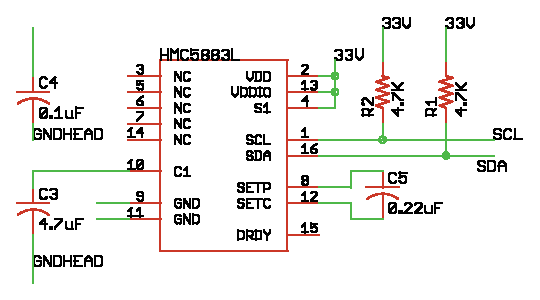
\includegraphics[width=0.5\textwidth]{figures/hmc5883LSchematic.eps}
 \end{figure}
 
 The HMC-5883L has an accuracy of 2 milliGauss on each axis, which corresponds to a accuracy.\\
 %todo:calc gauss to angles

 Both magnetometers were calibrated for bot soft-iron and hard-iron effects using a method documented in\cite{magCalibration}.
 To do this, data was acquired for one minute with the magnetometer being swept through all directions. An ellipsoid was fit to the data using a ordinary least squares method available from the Matlab file exchange\cite{ellipsoidFit}.
 The least squares fit estimates the center and radius of each axis. The center values for each axis are subtracted from the readings to remove hard-iron effects. Each $i$-th axis is then scaled by $\frac{1}{R_i}$ to ``squish" the ellipse into a circle, which removes soft-iron effects.
\subsection*{Euler Angle Kalman Filter}
For increased accuracy, a discrete linear Kalman filter is applied. This necessitated adding a three-axis gyroscope to the system. The gyroscope chosen was the Invensense ITG-3200, which comes in a QFN package. This gyroscope has a total error of $0.38^\circ/$s-rms\cite{itg3200DataSheet}, and uses a digital I$^2$C interface on a 3.3V operating voltage. The gyroscope has a full-scale span of $\pm2000^\circ/$s. The gyroscope was integrated into the main sensor board using a circuit based on that of Sparkfun's ITG-3200 breakout board\cite{itg3200BOBSchematic}.

\begin{figure}[h!]
  \caption{ITG-3200 Eagle Schematic} \label{itg3200Schematic}
  \centering
    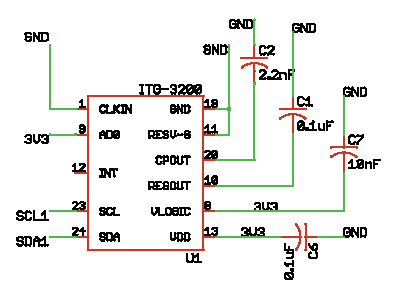
\includegraphics[width=0.6\textwidth]{figures/itg3200Schematic.eps}
\end{figure}

The gyroscope was calibrated using a two-step process similar to that of the accelerometer. First, zero-offset noise was removed from each axis by acquiring data for 10 seconds and subtracting the simple average from future readings. Second, the gyro was placed on a turn table which was set to $33 \frac{1}{3}$ RPM. Each axis was first lined up in the positive direction and next in the negative direction, and a linear fit was applied between the two data points.\\

With the angular rates available from the gyroscope, the system equations for the Kalman filter are
\begin{align}
\begin{bmatrix}
\phi_{k}\\
\theta_{k}\\
\psi_{k}
\end{bmatrix} & = \begin{bmatrix}
1 & 0 & 0\\0 & 1 & 0\\0 & 0 & 1
\end{bmatrix}\begin{bmatrix}
\phi_{k-1}\\
\theta_{k-1}\\
\psi_{k-1}
\end{bmatrix}
+ \begin{bmatrix}
\Delta T & 0 & 0 \\ 0 & \Delta T & 0\\0 & 0 & \Delta T
\end{bmatrix}\begin{bmatrix} 
p_k \\ q_k \\ r_k 
\end{bmatrix}+\hat{w}_{k-1}\\
z_k & = \begin{bmatrix}
1 & 0 &0\\0&1&0\\0&0&1
\end{bmatrix}\begin{bmatrix}
\phi_{k}\\
\theta_{k}\\
\psi_{k}
\end{bmatrix}+\hat{v}_{k-1}
\end{align}

The measurement covariance noise matrix was calculated using the standard deviation of the error between the magnetometer's ellipsoid fit and the acquired, calibrated data itself. The process noise covariance matrix was calculated using the standard deviation of the zero offset calibration data for the rate gyroscope.

\section{Wind Angles}
The accuracy at which the aerodynamic wind angles are calculated is critical to the overall prediction accuracy. In keeping with the goal of minimizing the number of required sensors, an attempt was made to estimate aerodynamic angles without directly measuring them. There has been a plethora of work conducted on this subject. One of the first available papers on the subject was from the Air Force Institute of Technology \cite{joseph1988}. In that paper, two methods were developed: one for in flight estimation, and the other for post-flight estimation. Both methods relied on either estimated or known stability derivatives. Since the purpose of this thesis is to estimate part of the dynamics, this estimating scheme will not work. Other techniques assume linearization about an operating condition \cite{morelli2012real}. For R/C aircraft this assumption generally cannot be made due to visual flight rules. Other work \cite{Lie2013} combined a dynamics model and a no-vertical-wind assumption. The overarching theme of this previous estimation work was that too many assumptions needed to be made to get results that were not accurate enough ($\approx1^\circ-2^\circ$) for drag polar estimation. For this reason, it was necessary to directly measure airflow angles.\\

A five-hole probe was chosen to measure aerodynamic angles as they do not contain moving parts and can provide very accurate, repeatable data. The five-hole probe selected was the Aeroprobe Air Data probe. It has a length of 6 inches and a diameter of 1/8 inch and comes calibrated to pressures.
%todo:document calibration process

 Each pair of lines of the air data probe is connected to an All Sensors digital differential pressure sensor with a full scale range of $\pm$5"-H$_2$O\cite{allsensorsDDO}.

\begin{figure}[H]
  \caption{All Sensors 5-INCH-D-DO Pressure Sensor} \label{allsensorsPressurePic}
  \centering
    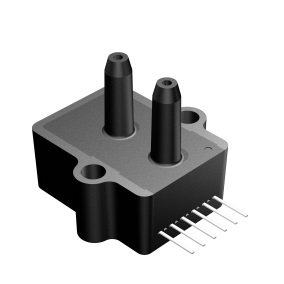
\includegraphics[width=0.5\textwidth]{figures/allsensorsPressure.jpg}
\end{figure}

These pressure sensors have a total error band of 0.25\% of full scale. They use a UART serial interface that operates on a 5V logic level, but the logic levels are compatible with the 3.3V interface of the Arduino Due. The serial interface includes addressable read commands, which allows multiples devices on a single bus, and ensures all devices record pressure at the same time. The sensor can output both a 14-bit pressure reading and a 12-bit temperature reading, which the devices uses to correct its pressure measurement.\\

The pressure sensors were calibrated using the same two step process as the gyroscope and accelerometer. The zero offset was obtained by connecting port A to port B and taking data for 10 seconds. Pressure was applied for the linear fit using a %todo:cite vacuum gun Russ uses to calibrate

\subsection{Wind Angle Kalman Filter}

To improve the accuracy of the wind angle estimation, a discrete Extended Kalman filter was used. The state transition functions are nonlinear and are
\begin{align}
\dot{\alpha} & = \frac{1}{V\cos\beta}(-a_x\sin\alpha+a_z\cos\alpha)+q-(p\cos\alpha+r\sin\alpha)\tan\beta\\
\dot{\beta} &=\frac{1}{V}(-a_x\cos\alpha\sin\beta+a_y\cos\beta-a_z\sin\alpha\sin\beta)+p\sin\alpha-r\cos\alpha
\end{align}

These state transition equations come from solving for the vehicle forces in wind axes instead of body axes\cite{klein2006aircraft}. The equations for the Kalman filter for the wind angles are
\begin{align}
\begin{bmatrix}
\alpha_k\\\beta_k
\end{bmatrix} &= \begin{bmatrix}
1& 0\\0&1
\end{bmatrix}\begin{bmatrix}
\alpha_{k-1}\\\beta_{k-1}
\end{bmatrix}+\begin{bmatrix}
\Delta T& 0\\0&\Delta T
\end{bmatrix}\begin{bmatrix}
\dot{\alpha_{k}}\\\dot{\beta_{k}}
\end{bmatrix}+\hat{w}_{k-1}\\
z_k & = \begin{bmatrix}
1 & 0\\0&1
\end{bmatrix}\begin{bmatrix}
\alpha_{k}\\
\beta_{k}
\end{bmatrix}+\hat{v}_{k-1}
\end{align}

The process covariance matrix was calculated using the error propagation discussed in Section \ref{pointErrorSection} and the standard deviation data from the zero offset calibration of each of the sensors. The measurement noise covariance matrix was calculated based on the standard deviation data for the zero offset pressure transducers connected to the five-hole probe.


\section{Additional Sensors}
A uBlox LEA-6T GPS receiver was included in the data acquisition system to aid in mission visualization. This model was selected for its ability to output raw timing data, which can potentially be used to get an extremely accurate inertial velocity estimate\cite{ubloxDemo}. The receiver itself was integrated onto a board sold by CGS Shop and has UART,USB, and I$^2$C interface options. 

\begin{figure}[H]
  \caption{CGS Shop Board for uBlox LEA-6T} \label{gpsPicture}
  \centering
    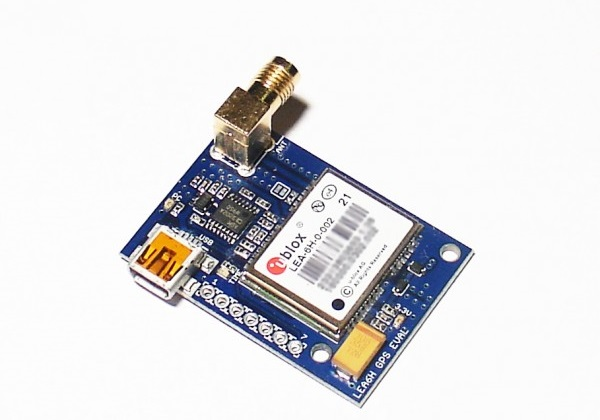
\includegraphics[width=0.5\textwidth]{figures/gpsBoard.jpg}
\end{figure}

A barometric altitude sensor was also included the data acquisiton system. The model chosen was an All Sensors BARO-DO, which has a range of 600 mBar to 1100 mBar\cite{allSensorsBaroDatasheet}. It has a nominal error of 1.0 mBar. It has the same packaging and communication protocol as the All Sensors 5-INCH-D-DO used for wind angle measurement, which simplified integration. It was calibrated to remove zero offset, but was not checked for linearity. The zero offset was removed by comparing the output data to a %todo:cite Russ's lab atmospheric pressure gauge.

A digital temperature sensor was combined with the barometric altitude sensor to estimate the air density.
\begin{figure}[H]
  \caption{Dallas Semiconductors' DS18B20 Digital Temperature Sensors} \label{ds18b20Picture}
  \centering
    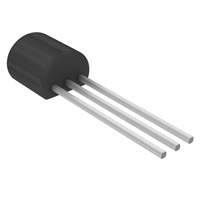
\includegraphics[width=0.25\textwidth]{figures/ds18b20Picture.jpg}
\end{figure}
 The DS18B20 from Dallas Semiconductors was chosen for its relatively simple One-Wire interface. The device can be powered with the communication line and has a $\pm$0.5$^\circ$C nominal accuracy\cite{DS18B20Datasheet}. It was calibrated across multiple measurements using the %todo:cite Russ's lab atmopsheric temp gauge.\\

Header pins capable of reading commanded PWM signals to servos were also added. Future work could include stability derivative estimation, and the header pins provide PWM measurement, which can map to servo angles, if it is assumed the servo is not stalled. 

\section{Data Acquisition Integration}
The hardware was initially built using a breadboard to ensure proper connections and to develop software. Once completed, sensors were packaged into a shield for the Arduino. This shield plugs directly into the Arduino, eliminating the need to disconnect and reconnect wiring. A board responsible for interfacing the main sensor board with the HMR-2300 was also developed, and connects to the main board with an RJ-11 cable. This allows the magnetometer to be placed with relative freedom within a vehicles fuselage. A third board was developed to integrate the pressure sensors with the main sensor board. This pressure board can be located near a wing tip and  provides expandability should additional sensors be desired in the future. It also interfaces the temperature sensor. Finally, all data was saved to a microSD card attached to the main sensor board. Data was saved in binary format for both increased speed and file size reductions. Once on the ground, the data is converted to meaningful values using a MATLAB parser.
